\documentclass[12pt]{article}
\usepackage{amsfonts, amssymb, amsmath, amsthm}
\usepackage[margin=1in]{geometry}
\usepackage{tikz}
\usetikzlibrary{patterns, decorations.pathreplacing, arrows.meta}

\pagestyle{myheadings}
\markright{Explainer: Rudin 4.2 --- Continuity and Closure\hfill}

\newcommand{\R}{\mathbb{R}}
\newcommand{\Z}{\mathbb{Z}}

\begin{document}

\begin{center}
    \textbf{\Large Continuity Preserves ``Closeness''}\\[0.5em]
    \large A visual guide to Rudin 4.2
\end{center}

\section{What Does $f(\overline{E}) \subset \overline{f(E)}$ Mean?}

In plain English: \textbf{if a point is near $E$, its image is near $f(E)$}.

\begin{center}
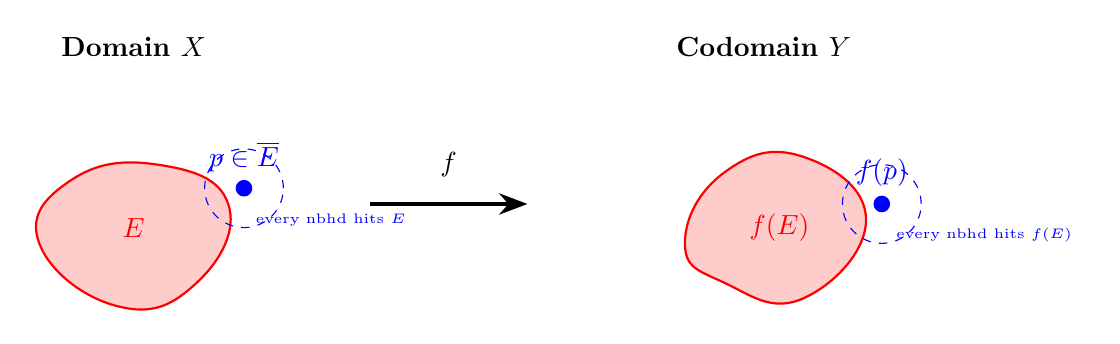
\begin{tikzpicture}[scale=1]
    % Domain side
    \begin{scope}[xshift=-4cm]
        \node at (0, 2.5) {\textbf{Domain $X$}};

        % Set E
        \draw[red, thick, fill=red!20] plot[smooth cycle, tension=0.8]
            coordinates {(-1.2,0) (-0.8,0.8) (0.3,1) (1.2,0.5) (0.8,-0.5) (-0.2,-0.8)};
        \node[red] at (0, 0.2) {$E$};

        % A point in closure(E) but not E
        \fill[blue] (1.4, 0.7) circle (3pt);
        \node[blue] at (1.4, 1.1) {$p \in \overline{E}$};

        % Show p is a limit point
        \draw[blue, dashed] (1.4, 0.7) circle (0.5);
        \node[blue, text width=2cm, align=center, font=\tiny] at (2.5, 0.3) {every nbhd hits $E$};
    \end{scope}

    % Arrow
    \draw[-{Stealth}, ultra thick] (-1, 0.5) -- (1, 0.5);
    \node at (0, 1) {$f$};

    % Codomain side
    \begin{scope}[xshift=4cm]
        \node at (0, 2.5) {\textbf{Codomain $Y$}};

        % Set f(E)
        \draw[red, thick, fill=red!20] plot[smooth cycle, tension=0.8]
            coordinates {(-1,0) (-0.5,0.9) (0.5,1.1) (1.3,0.3) (0.5,-0.7) (-0.5,-0.5)};
        \node[red] at (0.2, 0.2) {$f(E)$};

        % f(p) is in closure of f(E)
        \fill[blue] (1.5, 0.5) circle (3pt);
        \node[blue] at (1.5, 0.9) {$f(p)$};

        \draw[blue, dashed] (1.5, 0.5) circle (0.5);
        \node[blue, text width=2.5cm, align=center, font=\tiny] at (2.8, 0.1) {every nbhd hits $f(E)$};
    \end{scope}
\end{tikzpicture}
\end{center}

\textbf{Key idea:} Continuous functions can't ``jump away'' from a set. If $p$ is close to $E$, then $f(p)$ must be close to $f(E)$.

\section{Review: What is the Closure?}

The \textbf{closure} $\overline{E}$ of a set $E$ consists of:
\begin{itemize}
    \item All points \emph{in} $E$, plus
    \item All \emph{limit points} of $E$ (points that $E$ ``approaches'')
\end{itemize}

Equivalently: $p \in \overline{E}$ if and only if \textbf{every neighborhood of $p$ intersects $E$}.

\begin{center}
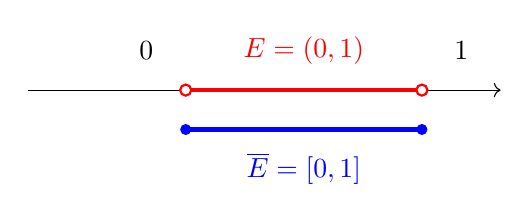
\begin{tikzpicture}[scale=1]
    \draw[->] (-1, 0) -- (5, 0);

    % E = (0,1)
    \draw[red, ultra thick] (1, 0) -- (4, 0);
    \draw[red, thick, fill=white] (1, 0) circle (2pt);
    \draw[red, thick, fill=white] (4, 0) circle (2pt);
    \node[red] at (2.5, 0.5) {$E = (0, 1)$};

    % Closure
    \fill[blue] (1, -0.5) circle (2pt);
    \fill[blue] (4, -0.5) circle (2pt);
    \draw[blue, ultra thick] (1, -0.5) -- (4, -0.5);
    \node[blue] at (2.5, -1) {$\overline{E} = [0, 1]$};

    \node at (0.5, 0.5) {$0$};
    \node at (4.5, 0.5) {$1$};
\end{tikzpicture}
\end{center}

\section{The Proof Strategy}

To show $f(\overline{E}) \subset \overline{f(E)}$:

\begin{enumerate}
    \item Pick any $p \in \overline{E}$ (so every neighborhood of $p$ hits $E$)
    \item Goal: show $f(p) \in \overline{f(E)}$ (every neighborhood of $f(p)$ hits $f(E)$)
    \item Use continuity as the bridge!
\end{enumerate}

\begin{center}
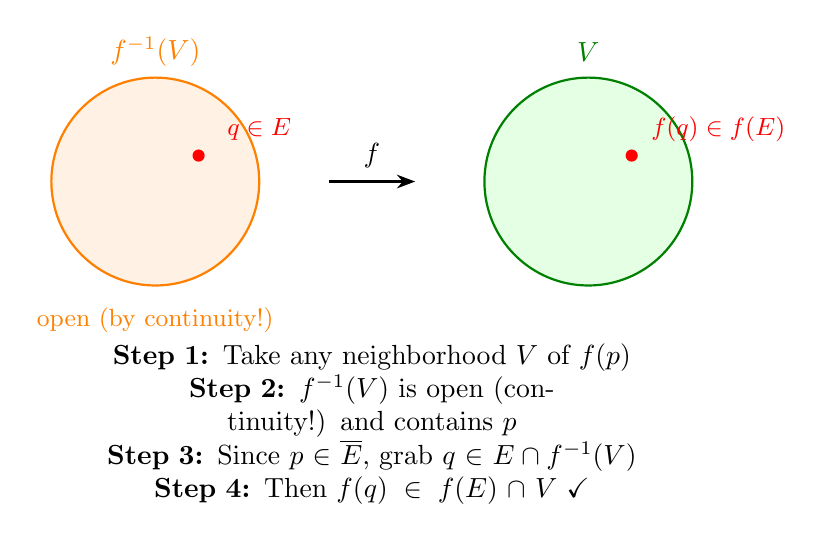
\begin{tikzpicture}[scale=1.1]
    % p and its preimage neighborhood
    \begin{scope}[xshift=-3.5cm]
        \fill[blue] (0,0) circle (2pt) node[below] {$p$};
        \draw[orange, thick, fill=orange!10] (0,0) circle (1.2);
        \node[orange] at (0, 1.5) {$f^{-1}(V)$};
        \node[orange, font=\small] at (0, -1.6) {open (by continuity!)};

        % Point q in E
        \fill[red] (0.5, 0.3) circle (2pt);
        \node[red, font=\small] at (1.2, 0.6) {$q \in E$};
    \end{scope}

    \draw[-{Stealth}, thick] (-1.5, 0) -- (-0.5, 0);
    \node at (-1, 0.3) {$f$};

    % f(p) and V
    \begin{scope}[xshift=1.5cm]
        \fill[blue] (0,0) circle (2pt) node[below] {$f(p)$};
        \draw[green!50!black, thick, fill=green!10] (0,0) circle (1.2);
        \node[green!50!black] at (0, 1.5) {$V$};

        % f(q) in f(E) cap V
        \fill[red] (0.5, 0.3) circle (2pt);
        \node[red, font=\small] at (1.5, 0.6) {$f(q) \in f(E)$};
    \end{scope}

    \node[text width=7cm, align=center] at (-1, -2.8) {
        \textbf{Step 1:} Take any neighborhood $V$ of $f(p)$\\
        \textbf{Step 2:} $f^{-1}(V)$ is open (continuity!) and contains $p$\\
        \textbf{Step 3:} Since $p \in \overline{E}$, grab $q \in E \cap f^{-1}(V)$\\
        \textbf{Step 4:} Then $f(q) \in f(E) \cap V$ \checkmark
    };
\end{tikzpicture}
\end{center}

\section{Why the Converse Fails}

The converse would say: $\overline{f(E)} \subset f(\overline{E})$.

\textbf{Translation:} ``Every point near $f(E)$ is the image of some point near $E$.''

This can fail when a continuous function ``sends points to infinity'' --- points of $f(E)$ accumulate at a value that $f$ never reaches.

\begin{center}
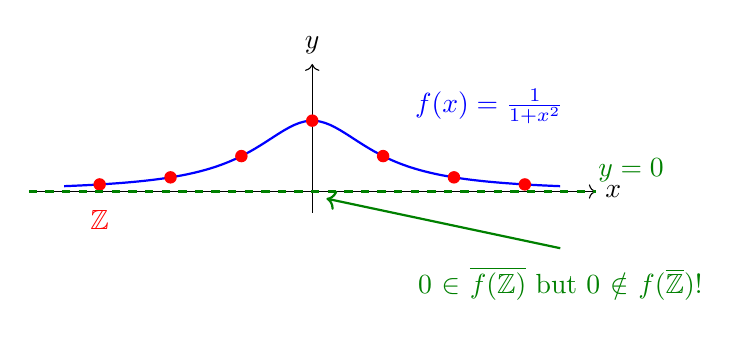
\begin{tikzpicture}[scale=0.9]
    % Draw the function 1/(1+x^2)
    \draw[->] (-4, 0) -- (4, 0) node[right] {$x$};
    \draw[->] (0, -0.3) -- (0, 1.8) node[above] {$y$};

    % Curve
    \draw[blue, thick, domain=-3.5:3.5, samples=100] plot (\x, {1/(1+\x*\x)});
    \node[blue] at (2.5, 1.2) {$f(x) = \frac{1}{1+x^2}$};

    % Integer points
    \foreach \n in {-3,-2,-1,0,1,2,3} {
        \pgfmathsetmacro{\y}{1/(1+\n*\n)}
        \fill[red] (\n, \y) circle (2.5pt);
    }

    % E = Z marked on x-axis
    \node[red] at (-3, -0.4) {$\mathbb{Z}$};

    % The value 0 that's approached but never reached
    \draw[green!50!black, dashed, thick] (-4, 0) -- (4, 0);
    \fill[green!50!black] (0, 0) circle (0pt);
    \node[green!50!black] at (4.5, 0.3) {$y = 0$};

    \draw[->, green!50!black, thick] (3.5, -0.8) -- (0.2, -0.1);
    \node[green!50!black, text width=4cm, align=center] at (3.5, -1.3) {$0 \in \overline{f(\mathbb{Z})}$ but $0 \notin f(\overline{\mathbb{Z}})$!};
\end{tikzpicture}
\end{center}

\textbf{Why it fails:}
\begin{itemize}
    \item $\overline{\mathbb{Z}} = \mathbb{Z}$ (integers are closed --- no limit points)
    \item $f(\mathbb{Z}) = \{1, 1/2, 1/5, 1/10, \ldots\}$ and these values approach $0$
    \item So $0 \in \overline{f(\mathbb{Z})}$
    \item But $f(x) = \frac{1}{1+x^2} > 0$ for all $x$, so $0$ is never in the image
    \item Therefore $0 \notin f(\overline{\mathbb{Z}}) = f(\mathbb{Z})$
\end{itemize}

The converse fails because $f$ ``uses up'' its domain approaching $0$ asymptotically but never getting there.

\section{Summary}

\begin{center}
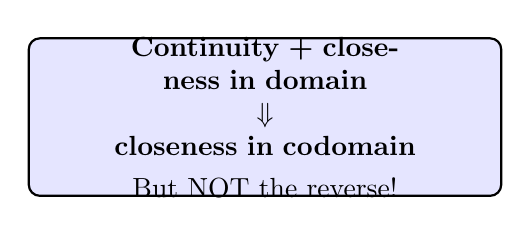
\begin{tikzpicture}
    \draw[thick, rounded corners, fill=blue!10] (-3, -1) rectangle (3, 1);
    \node[text width=5.5cm, align=center] at (0, 0) {
        \textbf{Continuity + closeness in domain}\\
        $\Downarrow$\\
        \textbf{closeness in codomain}\\[0.3em]
        But NOT the reverse!
    };
\end{tikzpicture}
\end{center}

\end{document}
